\documentclass[letterpaper, 10 pt, conference]{../ieeeconf} 
\IEEEoverridecommandlockouts
\overrideIEEEmargins
\pdfoptionpdfminorversion=4

\usepackage{amsmath}
\usepackage{mathtools}
\usepackage{textcomp}
\usepackage{graphicx}
\usepackage[font=footnotesize]{subcaption}
\usepackage[font=footnotesize]{caption}
\usepackage{hyperref}
\usepackage{amssymb}
\usepackage{booktabs}
\usepackage[normalem]{ulem}
\usepackage{verbatim}
\usepackage[export]{adjustbox}
\usepackage{amsmath}
\usepackage{url}
\usepackage{siunitx}
\usepackage[utf8]{inputenc}
\usepackage[TS1,T1]{fontenc}
\usepackage{array, booktabs}
\usepackage{caption}
\usepackage[cal=cm]{mathalfa}
\usepackage{algorithm}
\usepackage[noend]{algpseudocode}

% Labels in IEEE format
\newcommand{\eref}[1]{(\ref{#1})} % Equation
\newcommand{\sref}[1]{Sec.~\ref{#1}} % Section
\newcommand{\figref}[1]{Fig.~\ref{#1}} % Figure
\newcommand{\tref}[1]{Table~\ref{#1}} % Table
\newcommand{\aref}[1]{Algorithm~\ref{#1}} % Algorithm
\newcommand{\lref}[1]{Line~\ref{#1}} % Line
\renewcommand*\rmdefault{ppl}
\setlength{\textfloatsep}{5pt}

\usepackage{ifthen}
\usepackage[usenames,dvipsnames,table]{xcolor}
\newboolean{include-notes}
\setboolean{include-notes}{true} 
% http://en.wikibooks.org/wiki/LaTeX/Colors
\newcommand{\rhnote}[1]{\ifthenelse{\boolean{include-notes}}%
 {\textcolor{blue}{\textbf{RH: #1}}}{}}
\newcommand{\sanote}[1]{\ifthenelse{\boolean{include-notes}}%
 {\textcolor{green}{\textbf{SAN: #1}}}{}}

\begin{document}

% paper title
\title{6.857 Final Project: Milestone 5}
\author{Sebastiani Aguirre Navarro and Rachel Holladay}
\maketitle

\section{Introduction}
- set up the problem and outline the next several sections

\section{Data Set}
- introduce the data set, explain how dex net was generated and how we are going to use it

\section{Results}
- give the results from the architectures that we have

\section{Research Questions}

\subsection{Input Format}
our input versus what was used in the paper. also that other concatenated thing 

\subsection{Balancing Data Sets}
- number of positive versus negative examples

\subsection{Normalization}
- they normalized, should we

\subsection{Architecture Structure}
- list a couple different arch's

\section{Work Distribution}
- give basically same thing as before

\begin{comment}
\section{Initial Results}
\label{sec:results}
% “For milestone 4: Get an initial version of your system running end-to-end and produce initial results”

Our goal is to use machine learning techniques to predict the probability of successfully grasping an unknown object with a robotic arm.
We were forced to change our data set, for reasons explained in depth in \sref{sec:risk}, to the Dexerity Network (DexNet) 2.0 data set~\cite{mahler2017dex}.
We will first describe the input and output of our system and then describe some initial results. 
The DexNet 2.0 data set has 6.7 million synthetic point clouds with parallel-jaw grasps (a common robot hand type of two parallel fingers) and analytical grasp metrics. 

The data set covers 1,5000 3D object models used in DexNet 1.0~\cite{mahler2016dex} that are collected from a variety of other data bases and standardized with respect to position. 
Each object is paired with 2.5D point clouds, referred to as depth images, which are rendered with a variety of object and camera poses, where the camera intrinsics are known and used to center the depth image in a standardized fashion.
Each image is a black and white 32 by 32 pixel matrix. 
The parallel jaw grasps were sampled with rejection sampling for antipodal point pairs. 
The grasps are represented by a 7 dimensional vector specifying details of the grasp center, angle, object center and gripper width. 
Together the depth image matrix and grasp vector compose our input. 

Our label is given by the robust epsilon quality grasp metric (defined in~\cite{seita2016large}), which is thresholded by the value 0.002 to create binary labels.

For our initial results we sampled 10,000 data points from the 6.7 millon. 
Since the structure of the data changed considerably, pretrained models cannot be used since there is not an RGB component in the data. 
Therefore, we designed a simple Residual Network like the one shown in \figref{fig:network}. 
The idea is to pass the 32x32 depth maps through a ResNet with Batch Normalization to extract 1x8 features from it, and then these features are concatenated to the hand pose features that are passed to a fully connected layer that ouputs the likelihoods of each binary class. 
The training was carried in Keras~\cite{chollet2017keras}, using the RMSProp optimizer during 50 epochs with a batch size of 32 and 10\% of the dataset was used as Test. 
Given that we had a class imbalance of 1858 positive vs 8150 negatives in our datset subset, we assigned weights of 0.8 for positive and 0.2 for negative such that the underrepresented class could influnce training during each gradient descent step. 
This initial architecture did not work so well, however, since the error in the Test set was 81.0\%. 
If we observe the curves for loss and accuracy on Train and Validation during training in \figref{fig:loss} and \figref{fig:accuracy}, we can see that the network is overfitting. 

Moving forward, we have two ideas to address the overfitting issue.
The first is to create a more balanced training set with respect to the positive and negative labels. 
Another option is to reduce the model complexity and train on a smaller subset. 
We will also continue to experiment with network architecture, representations and metrics. 

\begin{figure*}[t!]
    \begin{subfigure}[t]{0.49\textwidth}
        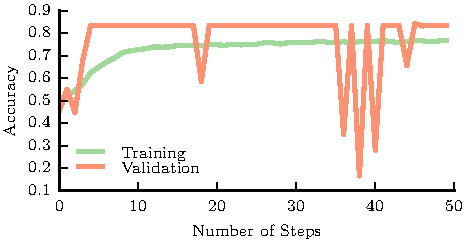
\includegraphics[width=0.99\columnwidth]{figs/accuracy.pdf}
        \caption{Accuracy} \label{fig:accuracy}
        \end{subfigure}
    \begin{subfigure}[t]{0.49\textwidth}
        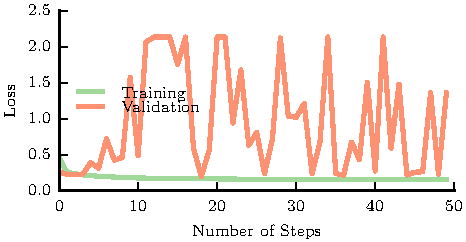
\includegraphics[width=0.99\columnwidth]{figs/loss.pdf}
        \caption{Loss} \label{fig:loss}
    \end{subfigure}
\caption{Initial Loss and Accuracy across the Training and Validation Sets} \label{fig:results}
\end{figure*}


\section{Risk Mitigation}
\label{sec:risk}
One of the risks we had mentioned in a previous milestone relating to data access unfortunately became realized. 
Early in our project we mentioned two possible datasets, the BigBird data set~\cite{singh2014bigbird} and the DexNet data set~\cite{mahler2017dex}.
We elected to use the BigBird data set in conjunction with the grasp generation and labeling process package "Grasp Pose Generator (GPG)" from~\cite{pas2017grasp}.
In attempting to create our training data, we realized that GPG did not directly use the data in the BigBird set and instead first performed a transformation that editted the depth files and generated surface normals. 
We were unable to find the opensource component that performed this transformation and the author of the report (at the time of this writing) has not replied to our request. 

Therefore, we have switched to using the DexNet 2.0 data set, whose data is described in further detail in \sref{sec:results}. 
If we are able to use the BigBird data set, we will consider using it in conjunction or as a comparison. 

\section{Division of Labor}

Rachel generated the training data from the DexNet data sets and set of the labeling mechanism. 
Sebastiani set up an environment in a AWS with GPUs, coded and trained initial Network In Network, Inception and ResNet based models in Keras/Tensorflow. 

\begin{figure}[t!]
    \centering
        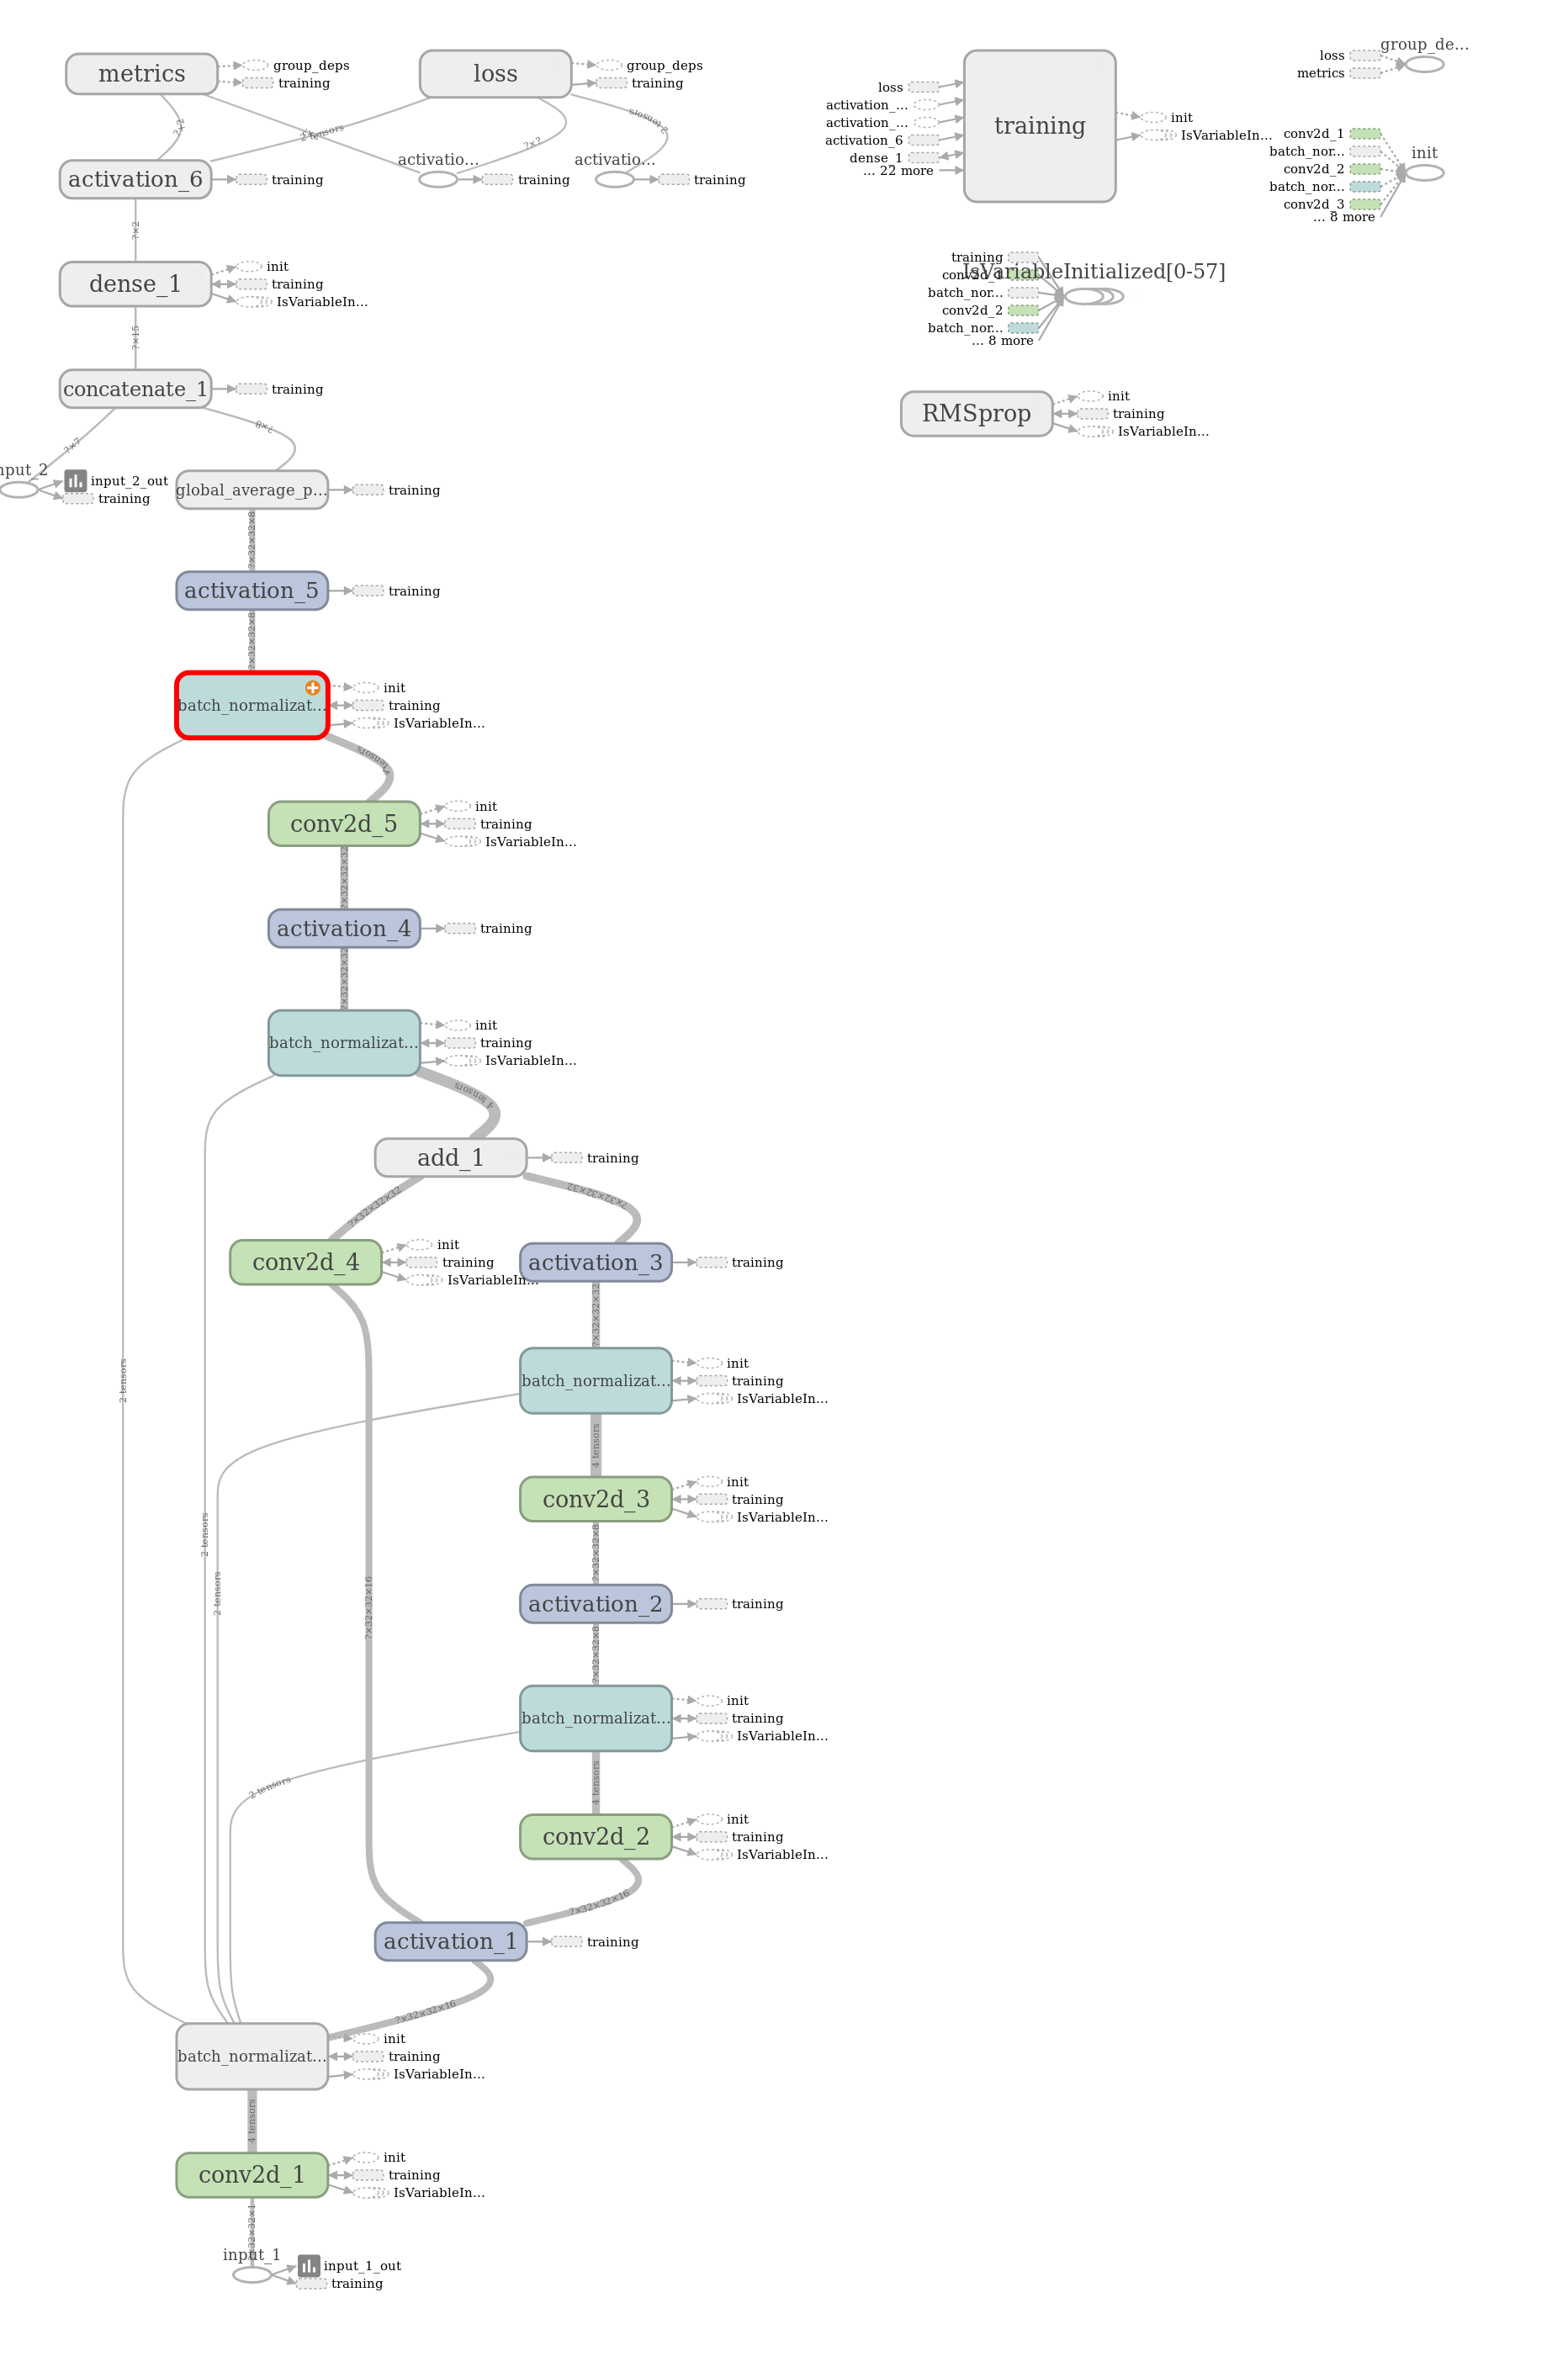
\includegraphics[width=0.7\columnwidth]{figs/dex_resnet.png}
    \caption{Network Structure} \label{fig:network}
\end{figure}
\end{comment}

{\footnotesize
    \bibliographystyle{ieeetr}
\bibliography{../references}}

\end{document}
